\documentclass[12pt]{article}
\usepackage{mandi}
\usepackage{braket}
\usepackage{graphicsx}
\usepackage{amsmath}
\usepackage{amsfonts}
\usepackage{tikz}
\usepackage{epstopdf}
\tolerance=1
\emergencystretch=\maxdimen
\hyphenpenalty=10000
\hbadness=10000
% Palatino font (ppl must be installed).
\renewcommand*\rmdefault{ppl}
% Iwona font (iwona must be installed).
%\renewcommand*\rmdefault{iwona}
\begin{document}
\title{Implementation of Quantum Computing Techniques on NMR systems}
\author{Anurag Pallaprolu \\ 2012B5A3405P \\ BITS Pilani }
\maketitle
\begin{abstract}
This document is submitted as a partial requirement for the course Quantum Information and Computing, BITS Pilani. The phenomenon of NMR can be used to generate spin states of nuclei and these can be used as qubits for computational purposes, the speciality being, an ensemble of molecules must be utilized. According to ~\cite{JAJ}, it is both the best, and the worst technologies in quantum computing, reasons being the ease at which unitary quantum gates can be implemented and the difficulty in exact measurements without disturbing the ensemble respectively. 
\end{abstract}
\clearpage
\section{Introduction}
\textbf{Nuclear Magnetic Resonance} is an important phenomenon in Physics, Chemistry and Medicine, was first discovered by \textbf{Isaac Isidor Rabi} in 1938, for which he won the Nobel Prize in 1944. Later, \textbf{Edward Mills Purcell} and \textbf{Felix Bloch} won the 1952 Nobel Prize \textit{for their developments of new methods for nuclear magnetic precision measurements and discoveries in connection therewith}.~\cite{npb}. The phenomenon occurs to certain nuclei, when placed in a strong static magnetic field, and are exposed to an oscillating magnetic field, depending on whether the nuclei possess intrinsic nucleonic spin or not. The concept of spin is quite simple as explained in the accompanying document ~\cite{me} and a fact that must be kept in mind is that we are talking about quantum mechanical version of spin and hence, we would be looking at things like Zeeman Effect etc,. When placed in a magnetic field of frequency $\mathbb{B}$, a particle with some net non-zero spin can absorb a photon of frequency $\nu$. The relationship being $$\nu = \gamma\mathbb{B}$$ The number $\gamma$ is called as the \textbf{gyromagnetic ratio} and depends on the particle at hand ~\cite{jph}. Simply seen, when any particle with a non zero spin is placed in a static magnetic field, it can stay in two energy levels, the lower energy level due to the straight pairing of N-S poles of the field to that of the particle, and the higher \textit{unstable} energy state of the anti-pairing of the N-S poles of the field with the particle.
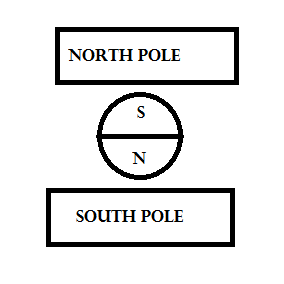
\includegraphics[scale=0.9]{nsns.png}
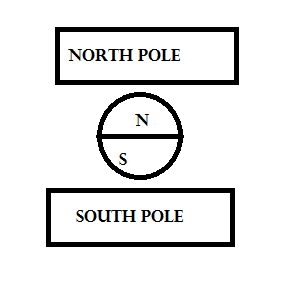
\includegraphics[scale=0.9]{nnss.png}

As we have seen, any transition from these two energy levels must be facilitated by quanta, according to Planck's hypothesis. Hence, we get the relation
$$E = h\gamma\mathbb{B}$$
When there is a lower level transition, or a photon arrives with the frequency equal to the \textbf{Larmor Frequency} given before, then a shift in the energy level happens~\cite{acadml}. In the case of \textbf{nuclear} magnetic resonance, the emission of photons or the absorbed photon usually lie in the radio frequency ranges of the electromagnetic spectrum. In NMR spectroscopy, $\nu$ is between 60 and 800 MHz for hydrogen nuclei. In clinical MRI, $\nu$ is typically between 15 and 80 MHz for hydrogen imaging ~\cite{jph}. The simplest possible implementation of NMR in actual atoms is the \textbf{Continuous Wave} NMR experiment. In this, you can either hold the magnetic field constant and supply RF pulses with varying frequency to note the absorbed energy, or, you can hold the pulsing frequency constant and vary the magnetic field to look for some resonance. The diagrams below should be helpful in making this point clear.

\begin{figure}
\begin{tikzpicture}[overlay]
\draw [<->,thick] (0,5) node (yaxis) [below] {Absorbed Energy}
        |- (5,0) node (xaxis) [right] {Frequency};
\draw [ultra thick, red] (0,0) -- (3,0)--(4,3)--(5,0)--(6,0);        
\end{tikzpicture}
\caption{The Energy-Frequency Diagram}
\end{figure}
\begin{figure}
\begin{tikzpicture}
\draw [<->,thick] (0,5) node (yaxis) [above] {Energy}
        |- (5,0) node (xaxis) [right] {Magnetic Field};

\draw (0,2.5) -- (4,4) --(6,4);
\draw (0,2.5) -- (4,1.5) --(6,1.5);
\draw [ultra thick, red] (3,1) -- (3,4);
\node [above] at (6,4) {Unpaired High Energy};
\node [above] at (6,1.5) {Paired High Energy};
\end{tikzpicture}
\caption{CWNMR Frequency Variation}
\end{figure}
\clearpage
\subsection{Ensemble}
Now, we shall move on to statistics of the spin particle ensembles. The problem with NMR spectroscopy is that the radio frequency photons are hard to detect, identify and measure as each one of them carries an energy of around $1\mu eV$. This leads to the following idea that, inorder to measure significant readings, an \textbf{ensemble} is required to be used experimentally. The number of molecules is approximated to be of the order of $10^{19}$ according to ~\cite{JAJ}. To analyze such large systems, we must comply to look at the \textit{macroscopic} point of view rather than the \textit{microscopic} one, and hence, we shall look at a bit of \textbf{Boltzmann statistics}. It is based on the probabilistic law that \textbf{Ludwig Boltzmann} proposed, and is very well explained in the standard ~\cite{Feyn}. We define $$\beta = \frac{1}{kT}$$ and then we can state from Boltzmann's law, that, 
$$\frac{N^{+}}{N^{-}} = e^{-\beta E}$$ where $N^+$ and $N^-$ are the number of particles in spin up and down states respectively and E is the energy difference between the two states. 
\begin{figure}
\begin{center}
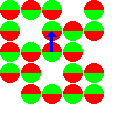
\includegraphics[scale=1]{ens1.png}
\end{center}
\caption{The Spin Packet of an Ensemble and the net $\mathbb{M}$ vector}
\end{figure}
Then, we take an ensemble and compartmentalize it into smaller boxes and call these \textbf{spin packets}. This then leads to the formulation of a magnetization vector $\mathbb{M}$ for each of these packets and it is obvious that $$\mathbb{M} =  \lambda (N^+ - N^-)$$ A system of axes can be set up here, with the z axis in the direction of $\mathbb{M}$. Let us take a deviation here, and look at the contributing Hamiltonian to NMR processes. According to the excellent paper ~\cite{ohio}, any atomic hamiltonian contains \textbf{nine important} terms that relate to any type of a quantum process. Let us look at them one by one. 
\clearpage
\subsection{The Atomic Hamiltonian}
The first one is called the \textbf{electronic Hamiltonian}, which is essentially a combination of all Coulombic potentials and kinetic energies
$$\mathcal{H}_{elec} = \sum_i \frac{{p_i}^{2}}{2m} - \sum_{i,j} \frac{z_je^2}{r_{ij}} + \sum_{i,j} \frac{e^2}{r_{ij}}$$
The next term is the \textbf{crystal field hamiltonian}, which deals with the interaction of electrons with the ions trapped in a crystal lattice. It also has a Coulombic form 
$$\mathcal{H}_{CF} = -\sum_{i,j} \frac{Q_je}{r_{ij}}$$
The third term is of great importance in particle physics, it is the \textbf{spin-orbit coupling hamiltonian}, which is of the form of 
$$\mathcal{H}_{SO} = \mu \mathbb{L}\mathbb{S}$$
where $\mathbb{L}$ and $\mathbb{S}$ are the orbital and spin angular momentum terms, respectively and $\mu$ is the \textbf{coupling constant} of the interaction, a term more commonly used in determining the extent of a force field in any quantum field theory. We shall not go deeper here. The next term, please. They are the \textbf{Zeeman Terms} which play an important role in describing, not only NMR but also another similar phenomenon by the name of \textbf{Electron Spin Resonance} or simply \textbf{ESR}.
$$H_{ESR} = \beta\vectdotvect{\mathbb{B}}{(\textbf{L}+\textbf{S})}$$
$$H_{NMR} = \mathcal{G}_{i}^n\beta^nB_{k}{\mathcal{N}^{ik}}$$
Here and henceforth, we will be using the Einstein summation convention of summing over repeated indices wherever found(the \textit{upstairs sums downstairs rule}). In the above equation $\mathcal{N}^{ik}$ is the $k$th component of the $i$th nucleus' magnetic moment. Indices which are not stairwise complementary are just for representation and are \textbf{not} summed over(like $n$ int the above equation).
The next hamiltonian is one that is important to NMR Computing, it is the \textbf{nuclear interaction hamiltonian}.
$$H_{NN} = \frac{1}{2}\mathcal{N}^\mu \mathcal{J}_{\mu \nu} \mathcal{N}^\nu $$
Here, the term $\mathcal{J}$ is a \textbf{tensorial} term representing the coupling coefficient between the two nuclei. More on this will be explained when we are looking at \textbf{qubit tensor product implementations} in NMR computers. The other three hamiltonians \textbf{the hyperfine splitting hamiltonian, spin-spin interaction hamiltonian, and the quadrupolar energy} are not exactly important here, and hence, I shall give references where it is explained much better.
Summarizing, any atomic hamiltonian will be of the form:
$$\mathcal{H}_{atom} = \sum_i \frac{{p_i}^{2}}{2m} - \sum_{i,j} \frac{z_je^2}{r_{ij}} + \sum_{i,j} \frac{e^2}{r_{ij}} -\sum_{i,j} \frac{Q_je}{r_{ij}} +\mu \mathbb{L}\mathbb{S} +  \beta\vectdotvect{\mathbb{B}}{(\textbf{L}+\textbf{S})} + \mathcal{G}_{i}^n\beta^nB_{k}{\mathcal{N}^{ik}} + \frac{1}{2}\mathcal{N}^\mu \mathcal{J}_{\mu \nu} \mathcal{N}^\nu $$
This equation is something big, and a few definitive \textit{relativistic} corrections~\cite{dirac} will make this theory complete.
\clearpage
\section{A Quick and Dirty Introduction to Quantum Computing Terminologies}
\subsection{Qubit}
I shall start out by explaining what a quantum bit or a \textbf{qubit} is. The name is self explanatory. Let me just point out the crucial difference, a classical bit can, at any point of time, take only one of the two quantized boolean states. Quantum bits on the other hand can be in a simultaneous superposition state of the individual quantized values. To put it symbolically,
\begin{center}
IN CLASSICAL COMPUTATION
\end{center}
$$\Ket{0}, \Ket{1}$$
\begin{center}
IN QUANTUM COMPUTATION
\end{center}
$$\frac{\Ket{0}+\Ket{1}}{\sqrt{2}}$$
 The $\sqrt{2}$ factor is completely arbitrary. In general, the two ket states might have any arbitrary (normalized) amplitudes. The behavior of these states is governed by the laws of quantum mechanics. That's all there is for a qubit. Now let us look at a few operations on qubits. They exist in vector spaces(more on this later) and can be operated on any two vectors. They could also be operated on each other using any standard vector arithmetic. An inner product can be established on the vector space in which the kets exist(more on this later).  The first question that might occur to any opportunistic person would be to expand this amalgamated state to more than one bit. This can be done due to the wonderful mathematical process of taking the \textbf{tensor product} or the \textbf{Kronecker product} of two or more qubits. The idea is quite simple and is exactly like the \textbf{direct product of two sets}. 
$$\frac{\Ket{0}+\Ket{1}}{\sqrt{2}}\otimes\frac{\Ket{0}-\Ket{1}}{\sqrt{2}} = \frac{1}{\sqrt{2}}(\Ket{00}-\Ket{01}+\Ket{10}-\Ket{11})$$
Your first thought might be, what in the world is $$\Ket{00}$$Well, don't get bewildered. Just think of it as a larger ket vector tracing two smaller qubit ket components. Let us talk about quantum gates to make this concept clear. 
\subsection{Quantum Gate}
A \textbf{gate} in any device is in general a logical unit which operates on Boolean variables. A \textbf{quantum gate} is a device which operates on \textit{quantum} boolean variables. I have to state a few facts before going into the explanation of the workings of a quantum gate. Every quantum mechanical operation takes one ket from the \textbf{Hilbert Space} in which it exists to another one with the help of a (matrix) transformation called as a \textbf{unitary transformation}. You might have heard of unitary matrices. Well, according to linear algebra, any linear transformation on a vector can be represented by a \textbf{matrix of transformation}. If this matrix turns out to be unitary, a situation which is most favorable for representing changes in quantum ket states, then it is a unitary transformation. This is a very bare bones version of one of the postulates of quantum mechanics. For a fuller explanation, refer to any standard quantum text like \textit{Griffiths}, \textit{Sakurai} or \textit{Shankar}. Anyway, any operation on a ket can be seen as a unitary matrix operating on its vector representation. Now, gates also operate on kets/qubits. Hence, the moral of the above story is that \textbf{every quantum gate can be represented in its unitary matrix representation}. For example, look at the simple circuit next page,\\
\begin{center}
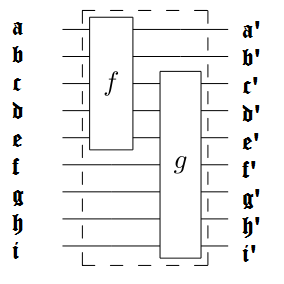
\includegraphics[scale=0.8]{qgate1.png}
\end{center}
The input lines all carry one qubit each. The gate $f$ operates on the first five lines and then the $g$ gate operates on the last seven lines. The input can be seen as a tensor product multi-qubit of 9 single qubits represented compactly as
$$\Ket{\Psi} = \bigotimes_{x=a}^{x=i}\Ket{x}$$ For instance, if each of the inputs was $\Ket{0}$, then $\Ket{\Psi} = \bigotimes_{x=a=0}^{x=i=0}\Ket{0}=\Ket{000000000}$. As discussed before, \textit{the operation of the $f$ gate can be represented by a unitary transformation on the initial (multi)ket}. Let us call this matrix as $\mathcal{F}$. Then the next state of the combined qubit after the $\mathcal{F}$  would then be $$\mathcal{F}\bigotimes_{x=f,x'=a}^{x=i,x'=e}\Ket{x'}\Ket{x} = \bigotimes_{x=f,x'=a}^{x=i,x'=e}\mathcal{F}\Ket{x'}\Ket{x}$$ Note the change in the indices of summation as not all individual qubits are going through $\mathcal{F}$. Let's call the multiqubit at this step as $\Ket{\Psi_{1}}$.The next step would be to operate $g$ onto the qubits $c$ through $i$. Let's call its matrix as $\mathcal{G}$. The qubit at this stage would be $$\mathcal{G}\Ket{\Psi_{1}} =  \bigotimes_{x=f,x'=a}^{x=i,x'=e}\mathcal{F}\Ket{x'}\mathcal{G}\Ket{x}$$
$$\bigotimes_{x=f,x'=a}^{x=i,x'=e}\mathcal{F}\Ket{x'}\mathcal{G}\Ket{x} = \bigotimes_{x=a'}^{x=i'}\Ket{x}$$
The concept of parallelism should get a bit clear now as you can clearly see the individual operation of gates on qubit, but the final (unnormalized) state is correlated. This should also point out one of the major issues with parallelism theory, \textit{we can compute a state in \textbf{one} step which contains, say, the values of the function $f(x)$ for many values of $x$(whereas a classical computer would take $n$ steps where $n$ is the number of values of $x$). But to access the values, we have to perform a measurement, and a measurement performed on a particular $\Ket{x}$ would lead to the \textbf{collapse of the ket at the value}}. The last line quantum mechanically tells us that we would lose information about all other values of $x$  but retain the value of $f(x_{measured})$. This might sound like quantum computing just lost a point against its classical opponent, but where it wins is (as we shall see in Deutsch's Algorithm next) the final state can be a combination of operated individual values, like $f(x_1)+f(x_2)$ etc., which the classical computer \textbf{would still take $n$ steps to do(in the present case 2)}. You can read up more on standard quantum gates from \textit{Nielson and Chuang}, but I think this discussion shall suffice for the documentation.
\subsection{Walsh-Hadamard Transform}
However, I shall describe one specific type of gate, called the \textbf{Hadamard Gate} named after Jacques Hadamard. It is represented by the symbol 
\begin{center}
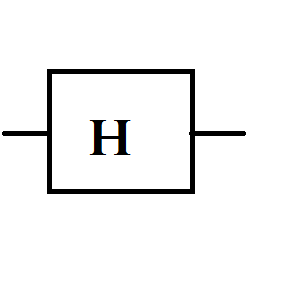
\includegraphics[scale=0.5]{qhad.png}
\end{center}
Simply put, let us take any qubit in the standard basis of $\mathbb{H}$ say $\Ket{\psi} = \alpha\Ket{0} + \beta\Ket{1}$. The operation of $\mathcal{H}$ on standard basis qubits is known $$\mathcal{H}\Ket{0} = \frac{\Ket{0}+\Ket{1}}{\sqrt{2}}$$
$$\mathcal{H}\Ket{1} = \frac{\Ket{0}-\Ket{1}}{\sqrt{2}}$$
With this, now we can see
$$\mathcal{H}\Ket{\psi} = \alpha\frac{\Ket{0}+\Ket{1}}{\sqrt{2}} + \beta\frac{\Ket{0}-\Ket{1}}{\sqrt{2}} = \frac{\alpha + \beta}{\sqrt{2}}\Ket{0} + \frac{\alpha - \beta}{\sqrt{2}}\Ket{1}$$
Hence, as you can see, the operation is quite simple, and one can easily derive the transformation matrix of $\mathcal{H}$. Now, let us take two qubits, for simplicity, let both of them be $\Ket{0}$. Now, let us apply the \textbf{Hadamard Gate on 2 Qubits or the Nth order Hadamard Gate} represented by $\mathcal{H}^{\bigotimes 2}$. This is nothing but the operator $\mathcal{H}\bigotimes\mathcal{H}$. Thus, two Hadamard gates operate on individual qubits and are again \textit{tensorially} combined into one qubit. Note the pattern of $\mathcal{H}^{\bigotimes n}$ as $n$ increases, as given below.
$$\mathcal{H}^{\bigotimes 2}\Ket{00} = \mathcal{H}\Ket{0}\mathcal{H}\Ket{0} = \frac{\Ket{00}+\Ket{01}+\Ket{10}+\Ket{11}}{2}$$
$$\mathcal{H}^{\bigotimes 3}\Ket{000} = \frac{\Ket{000}+\Ket{001}+....+\Ket{101}+\Ket{111}}{2^{3/2}}$$ Notice how all the binary numbers upto $2^n$ are being listed in the combined multikets. This general Hadamard Transform of $n$ qubits can be combined mathematically as
$$\mathcal{H}^{\bigotimes n}\Ket{0^n} = \sum_{x=0}^{x=2^n-1}\frac{\Ket{x}}{\sqrt{2^n}}$$ This operation is much more generally known as the \textbf{Walsh-Hadamard Transform} and comes under a general class of such summable or integrable transforms known as \textit{Fourier Transforms}, which can be proven to be convergent and are applicable for discontinuous functions as well(\textit{Dirichlet's Theorem}), but we shall not go into this much deep. The development of the neccesary tools is complete, we shall start our progress in the implementation of quantum computing systems in NMR experiments.
\section{Implementation}
\subsection{The Bloch Vectors, The Ket and The $\mathbb{SU}(2)\hom\mathbb{SO}(3)$}
To look at the implementation schema, we must first look at a bit of \textbf{representation} theory first. Any qubit can 
\bibliographystyle{plain}
\bibliography{nmrqc}
\end{document}